\appendix
\chapter{Appendix}

	\section{Parameters of Comsol model}
    \label{app:comsolParams}
    Comsol model for applying the interface shifting to pulsing in microwell devices (chapter \ref{chap:microculturePulses}) used the following physics modules:
    \begin{itemize}
    \item `Transport of diluted species' where the boundary condition at the inlets was set to `concentration' with \(0M\) and \(1M\) for the blank and drug inlets, respectively. An `outflow' boundary condition was used for the outlet.

    \item `Creeping flow' where the boundary condition at the inlets was set to `velocity' with values \(mediaFlow\) and \(0.05\cdot mediaFlow\) for the blank and and drug inlets, respectively. To apply the pulse, at time \(t=1s\) these values were flipped for \(p\_width\) with a \(300ms\) linear transition period (see section \ref{sec:pulses:comsol}). The outlet boundary condition was set to `pressure' with \(0mbar\).
    \end{itemize}

    Specific parameters are given in the following table:

    \begin{tabular}{l l p{5cm}}
        \textbf{Symbo}l & \textbf{Description} & \textbf{Value} \\ \hline \hline
        \(D\_c\) & Diffusion coefficient (small molecule)      & \(3\times 10^{-10}\frac{m^2}{s}\) \\
        \(w\_c\) & Channel width  & \(1.5mm\)         \\
        \(h\_c\) & Channel height & \(0.04mm\)        \\
        \(w\_i\) & Inlet width    & \(0.8mm\)        \\
        \(l\)   & Channel length & \(10mm\)        \\
        \(w\_mw\) & Microwell diameter & \(0.675mm\) \\
        \(h\_mw\) & Microwell depth    & \(0.12\), \(0.08\) or \(0.01mm\) \\
        \(d\_mw\) & Microwell distance from channel appex & \(0.15mm\) \\
        \(mediaFlow\) & Base flow rate & \(6\), \(12\), \(24\), \(36\frac{\mu l}{min}\) \\
        \(p\_width\) & Pulse width & \(1.5s\) or a range of pulse widths around this value normalized to the flow rate for finding
                                             the optimum (section \ref{sec:pulses:fastPulses}). \\
    \end{tabular}
        %       \begin{figure}[h]
 %           \centering
  %          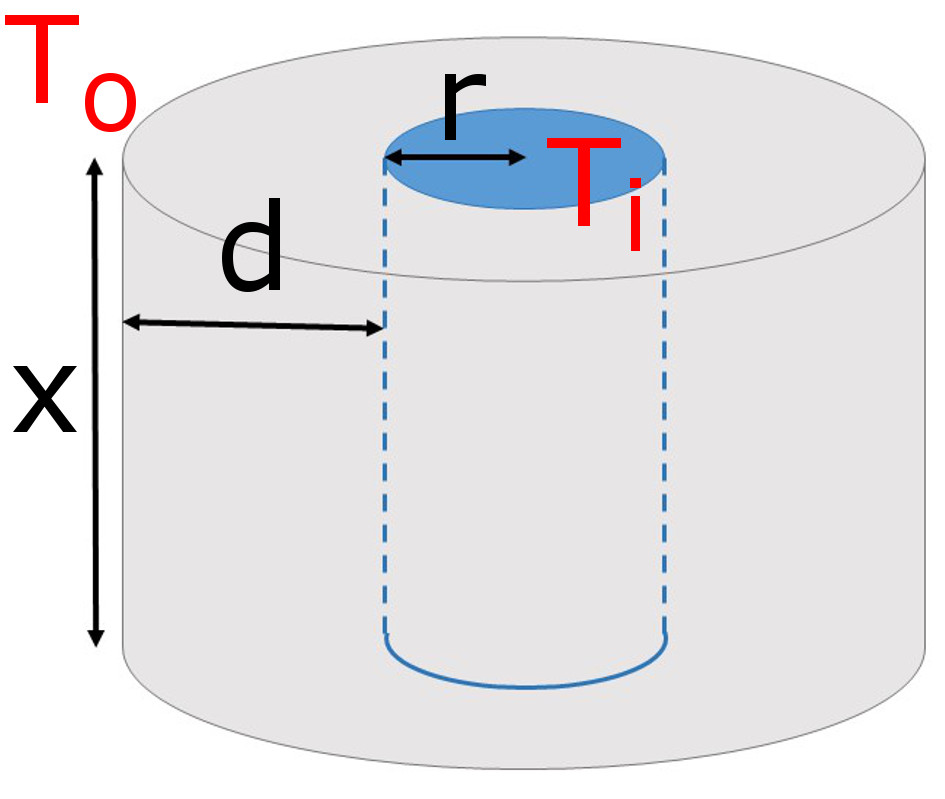
\includegraphics[width=4cm]{appendix/tubeIllustration/tubeIllustration.jpg}

   %         \label{fig:app:tubeIllustration}
    %    \end{figure}
\newpage
\section{MEA channel layouts}
       \begin{figure}[!h]
            \centering
            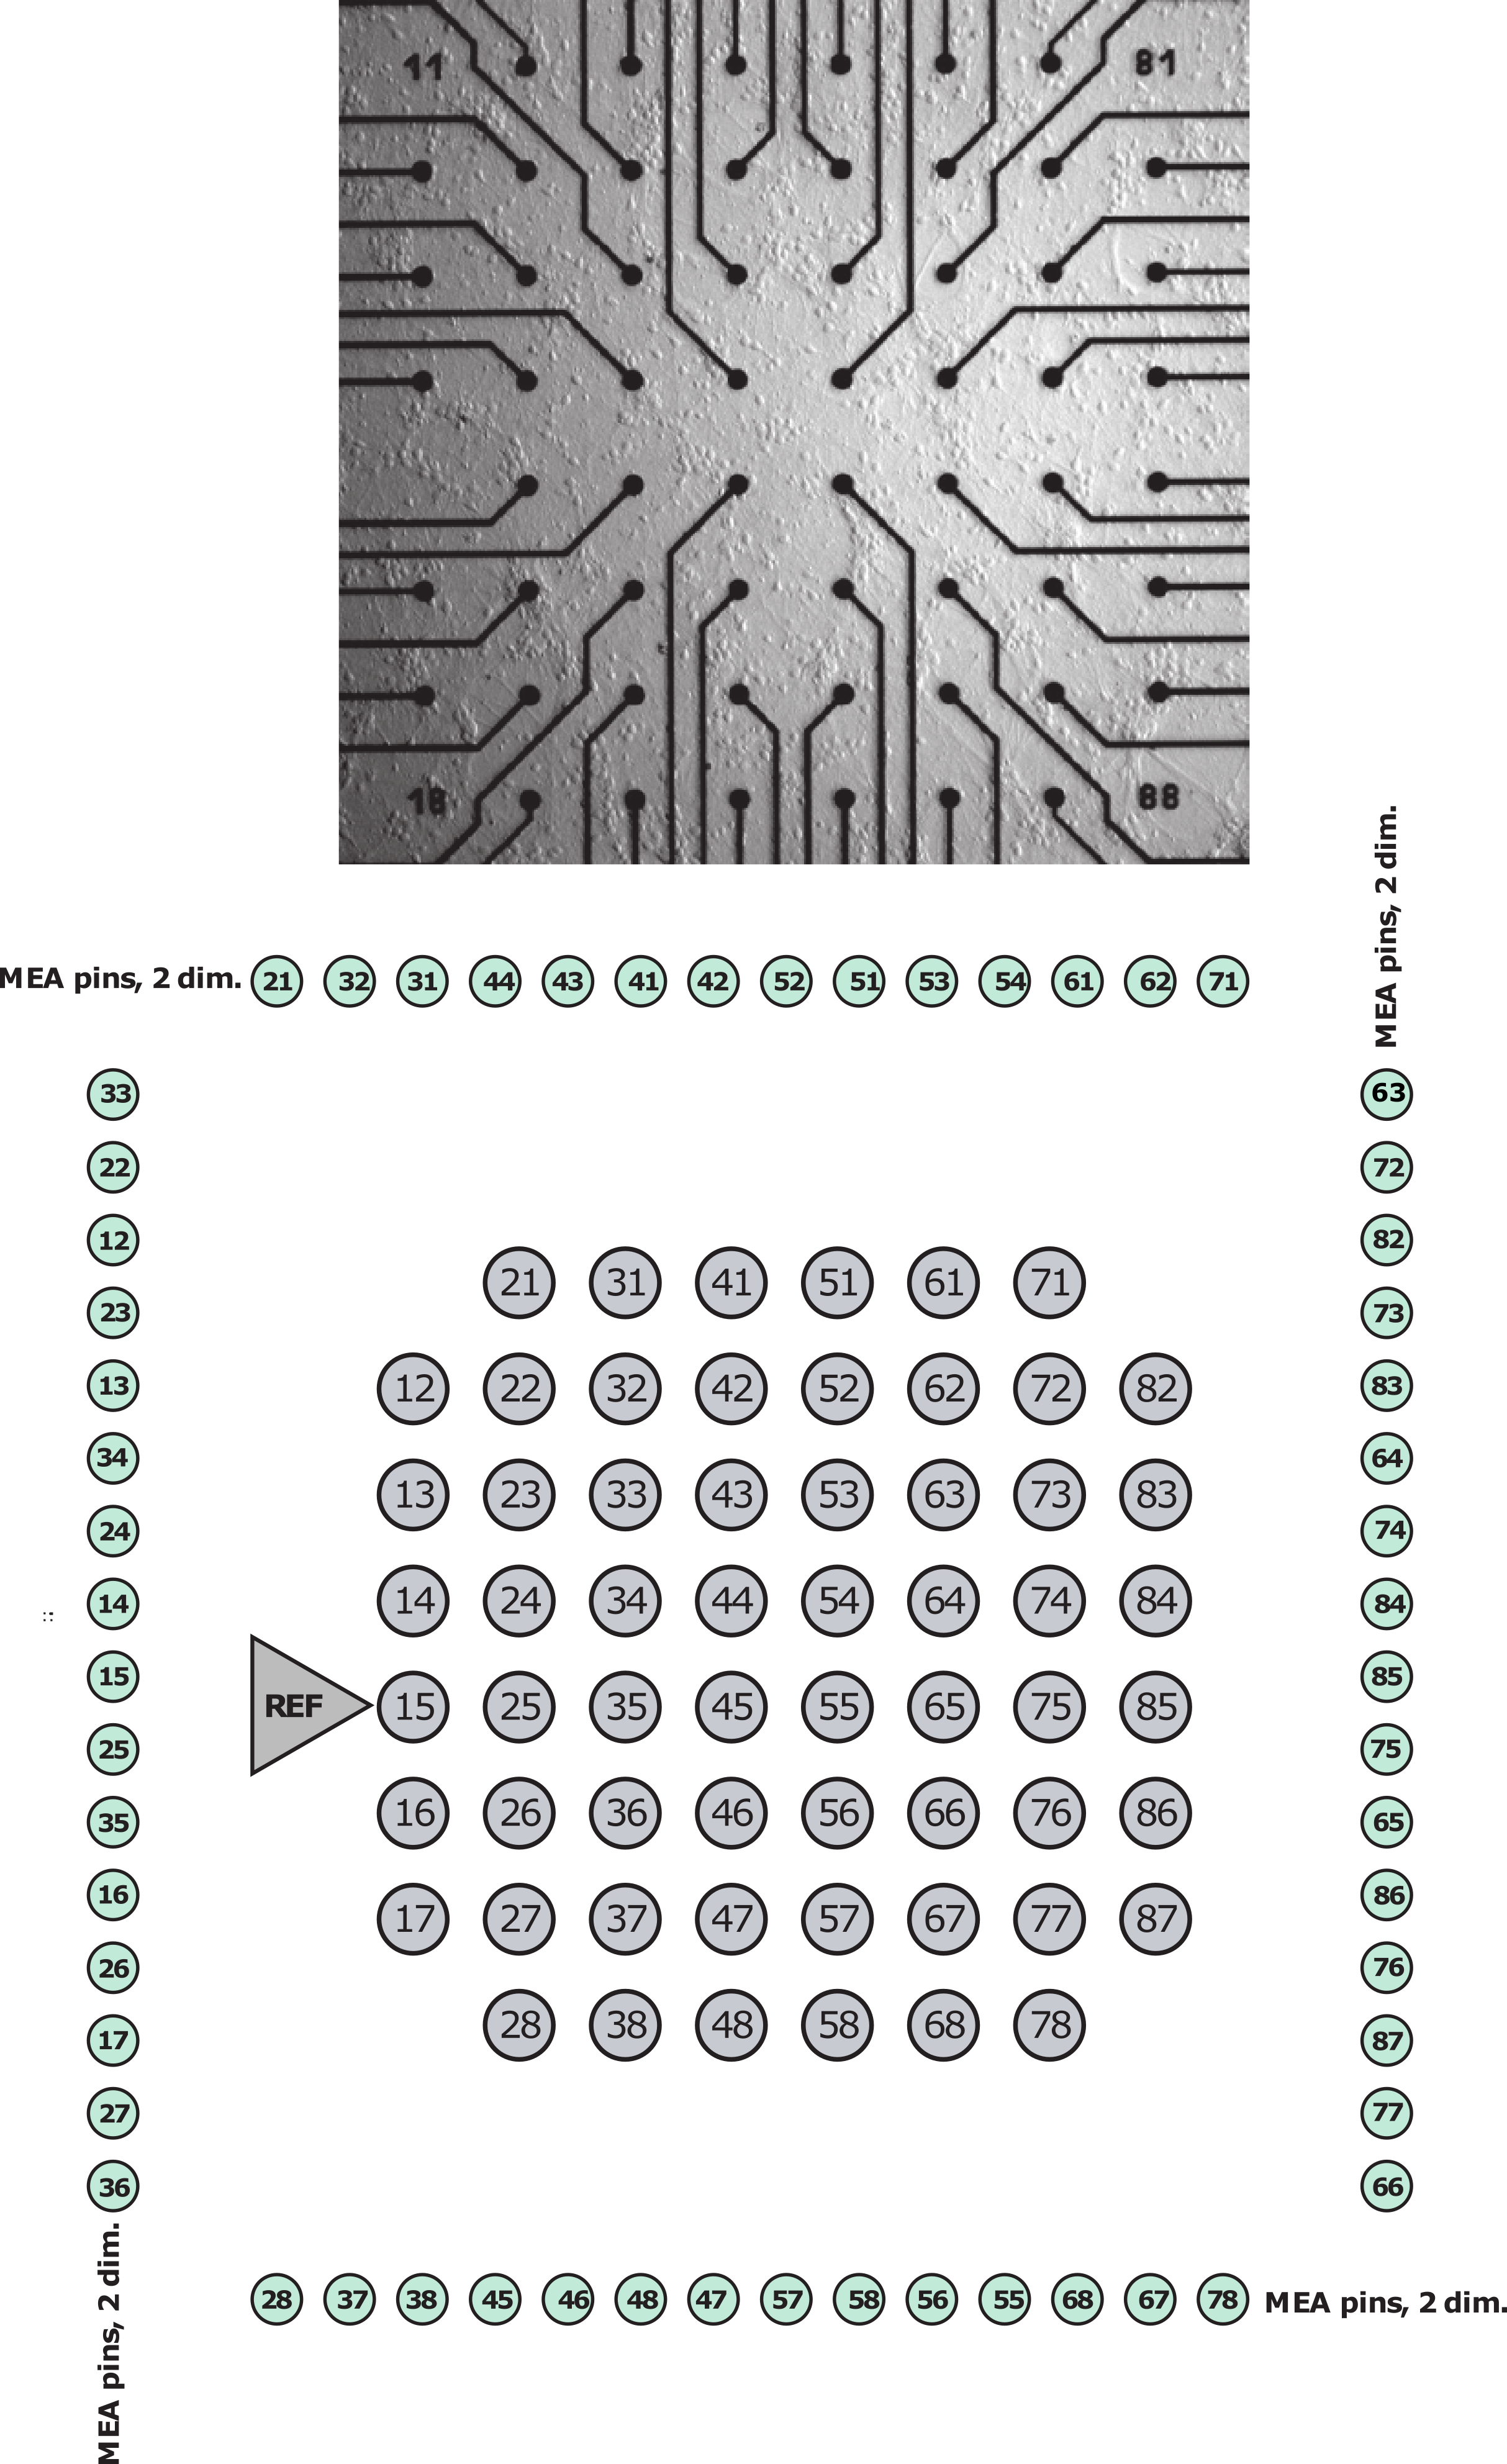
\includegraphics{appendix/8x8Layout.png}
            \caption[Spatial organization of MEA channel indexing for the \(8\times 8\) layout]{\textbf{Spatial organization of MEA channel indexing for the \(8\times 8\) layout.} In the case of the \(8 \times 8\) layout, the channel indexing represents a 2-dimensional coordinate system pointing to the spatial position of the indexed electrode (column then row).}
            \label{fig:app:8x8Layout}

        \end{figure}
\newpage
        \begin{figure}[!h]
            \centering
            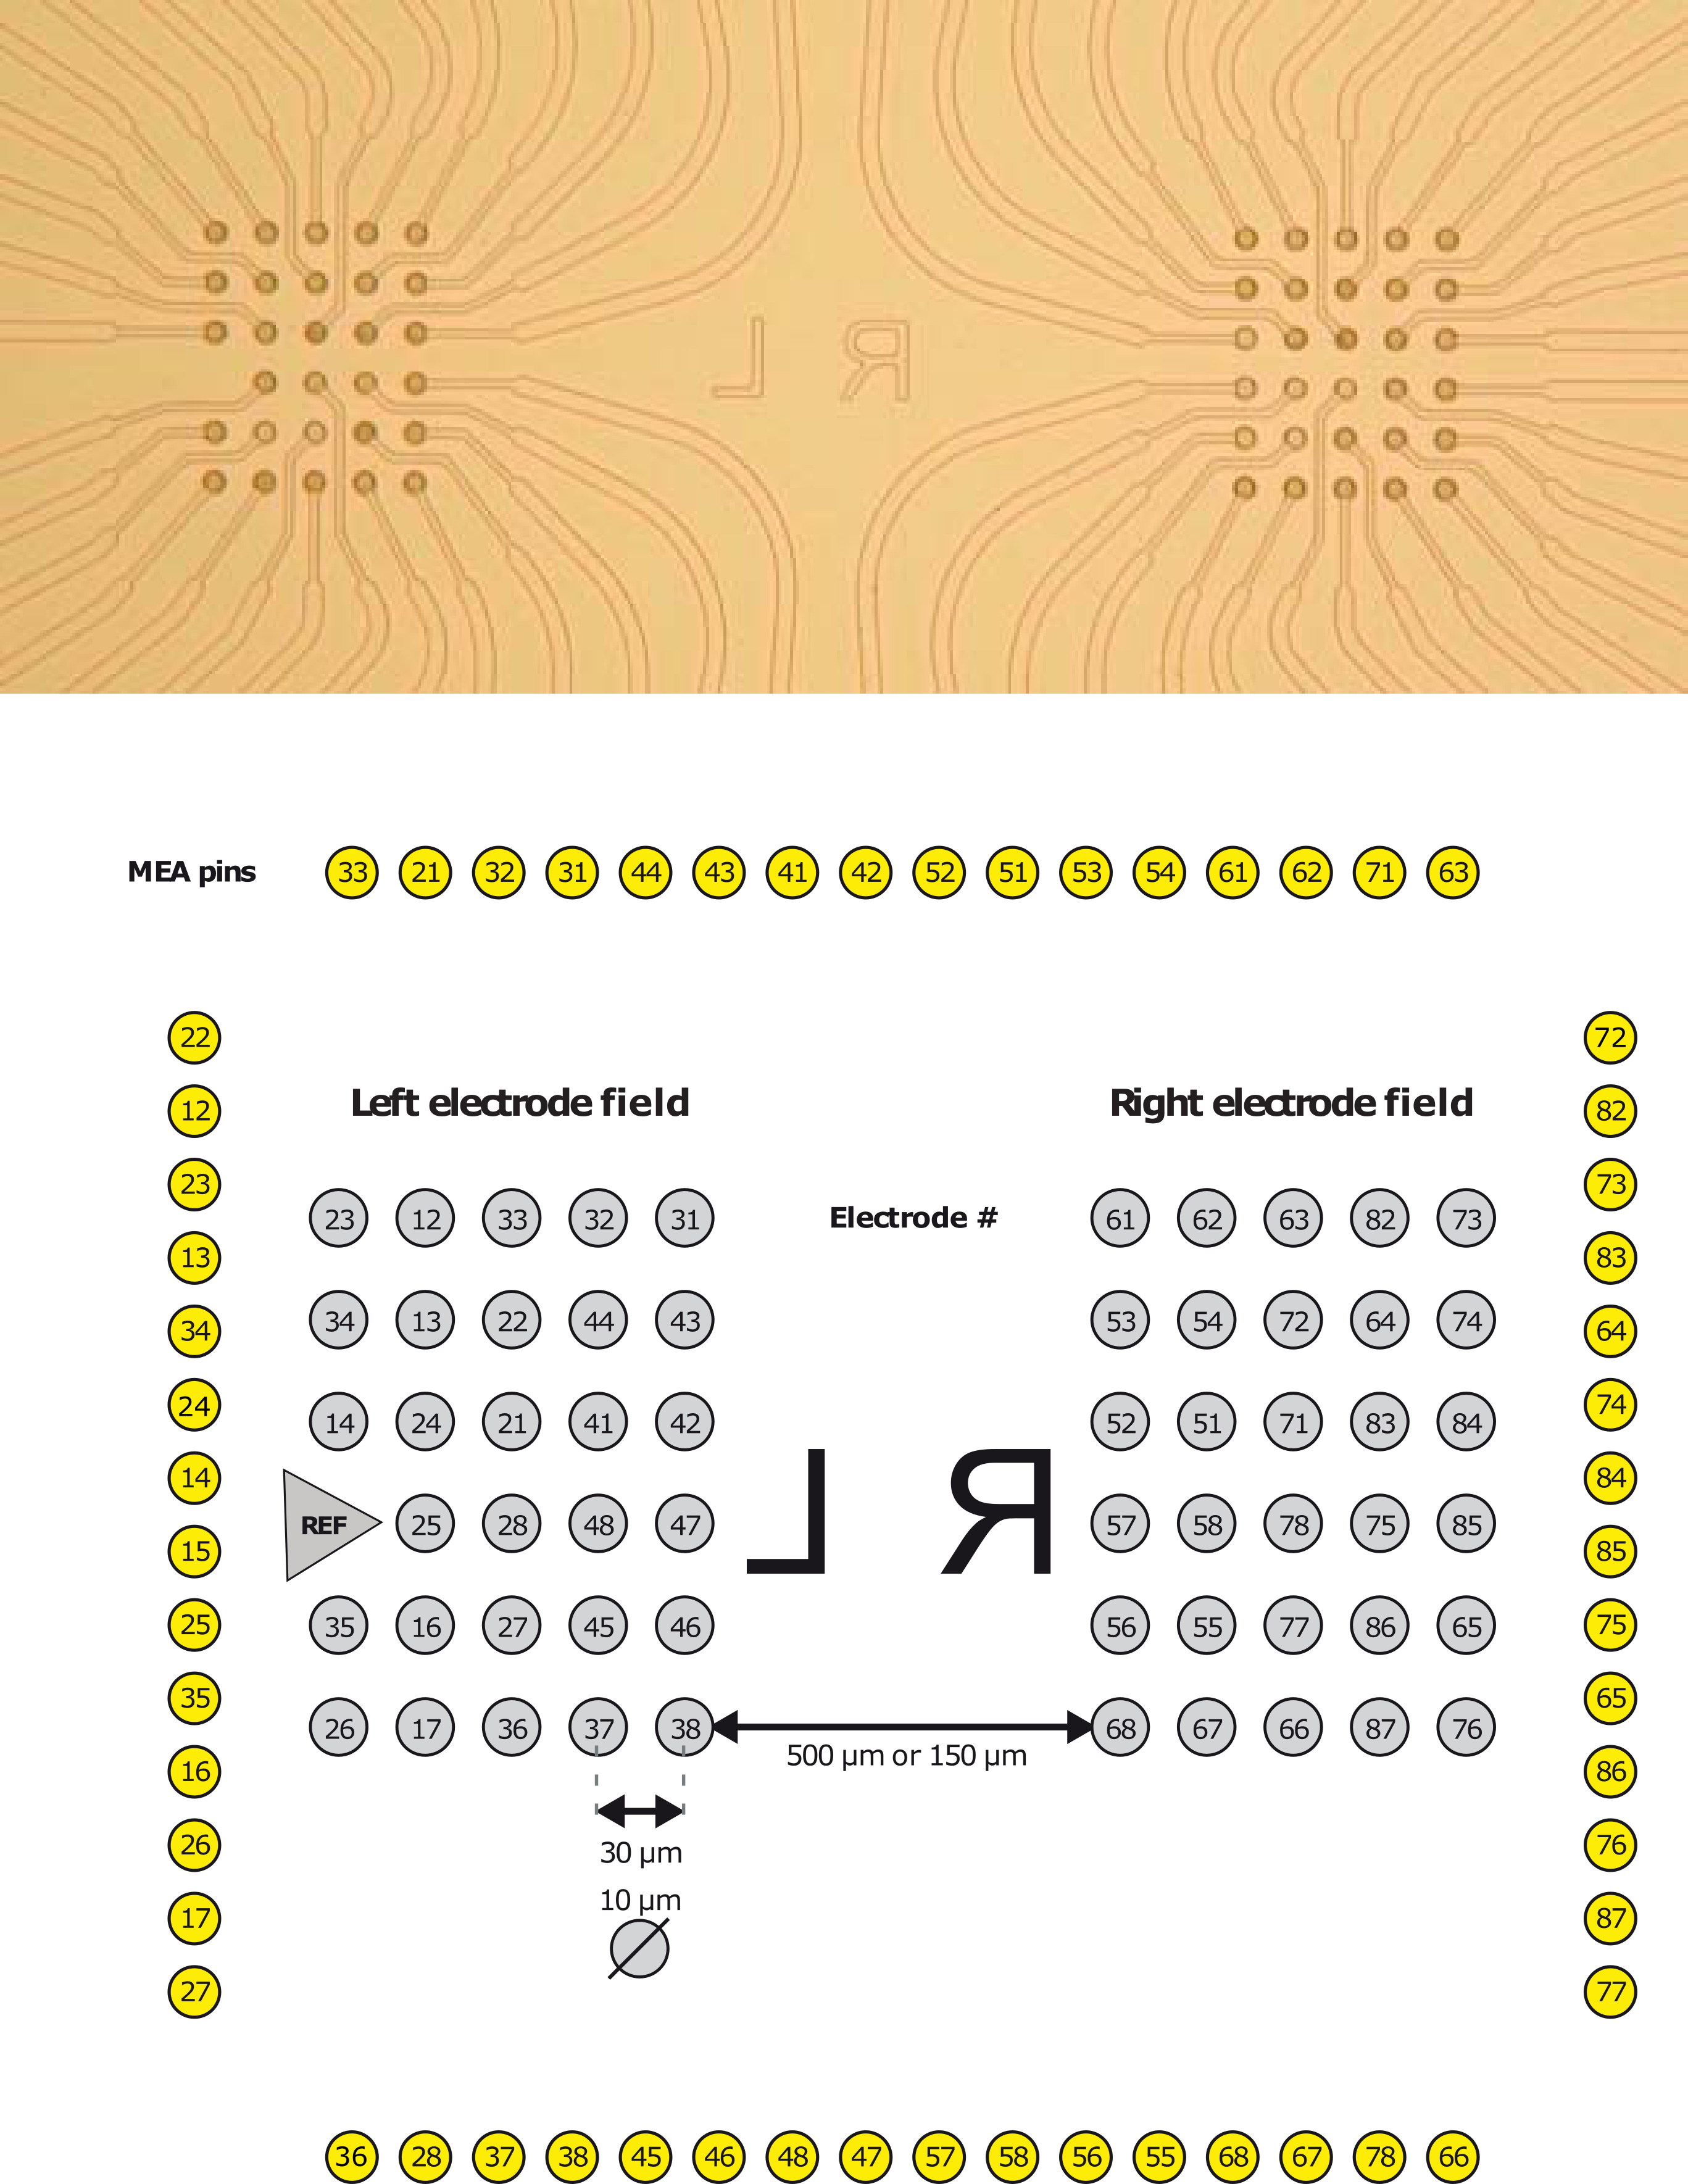
\includegraphics{appendix/HDLayout.png}
            \caption[Spatial organization of MEA channel indexing for the HD layout]{\textbf{Spatial organization of MEA channel indexing for the HD layout.} In the case of the HD layout, the channel indexing does not represent the spatial organization of the electrodes (with the reason being that it is historically bound to the original \(8 \times 8\) layout).}
            \label{fig:app:HDLayout}

        \end{figure}

\newpage

\section{Supplementary images and figures}
        \begin{figure}[!h]
            \centering
            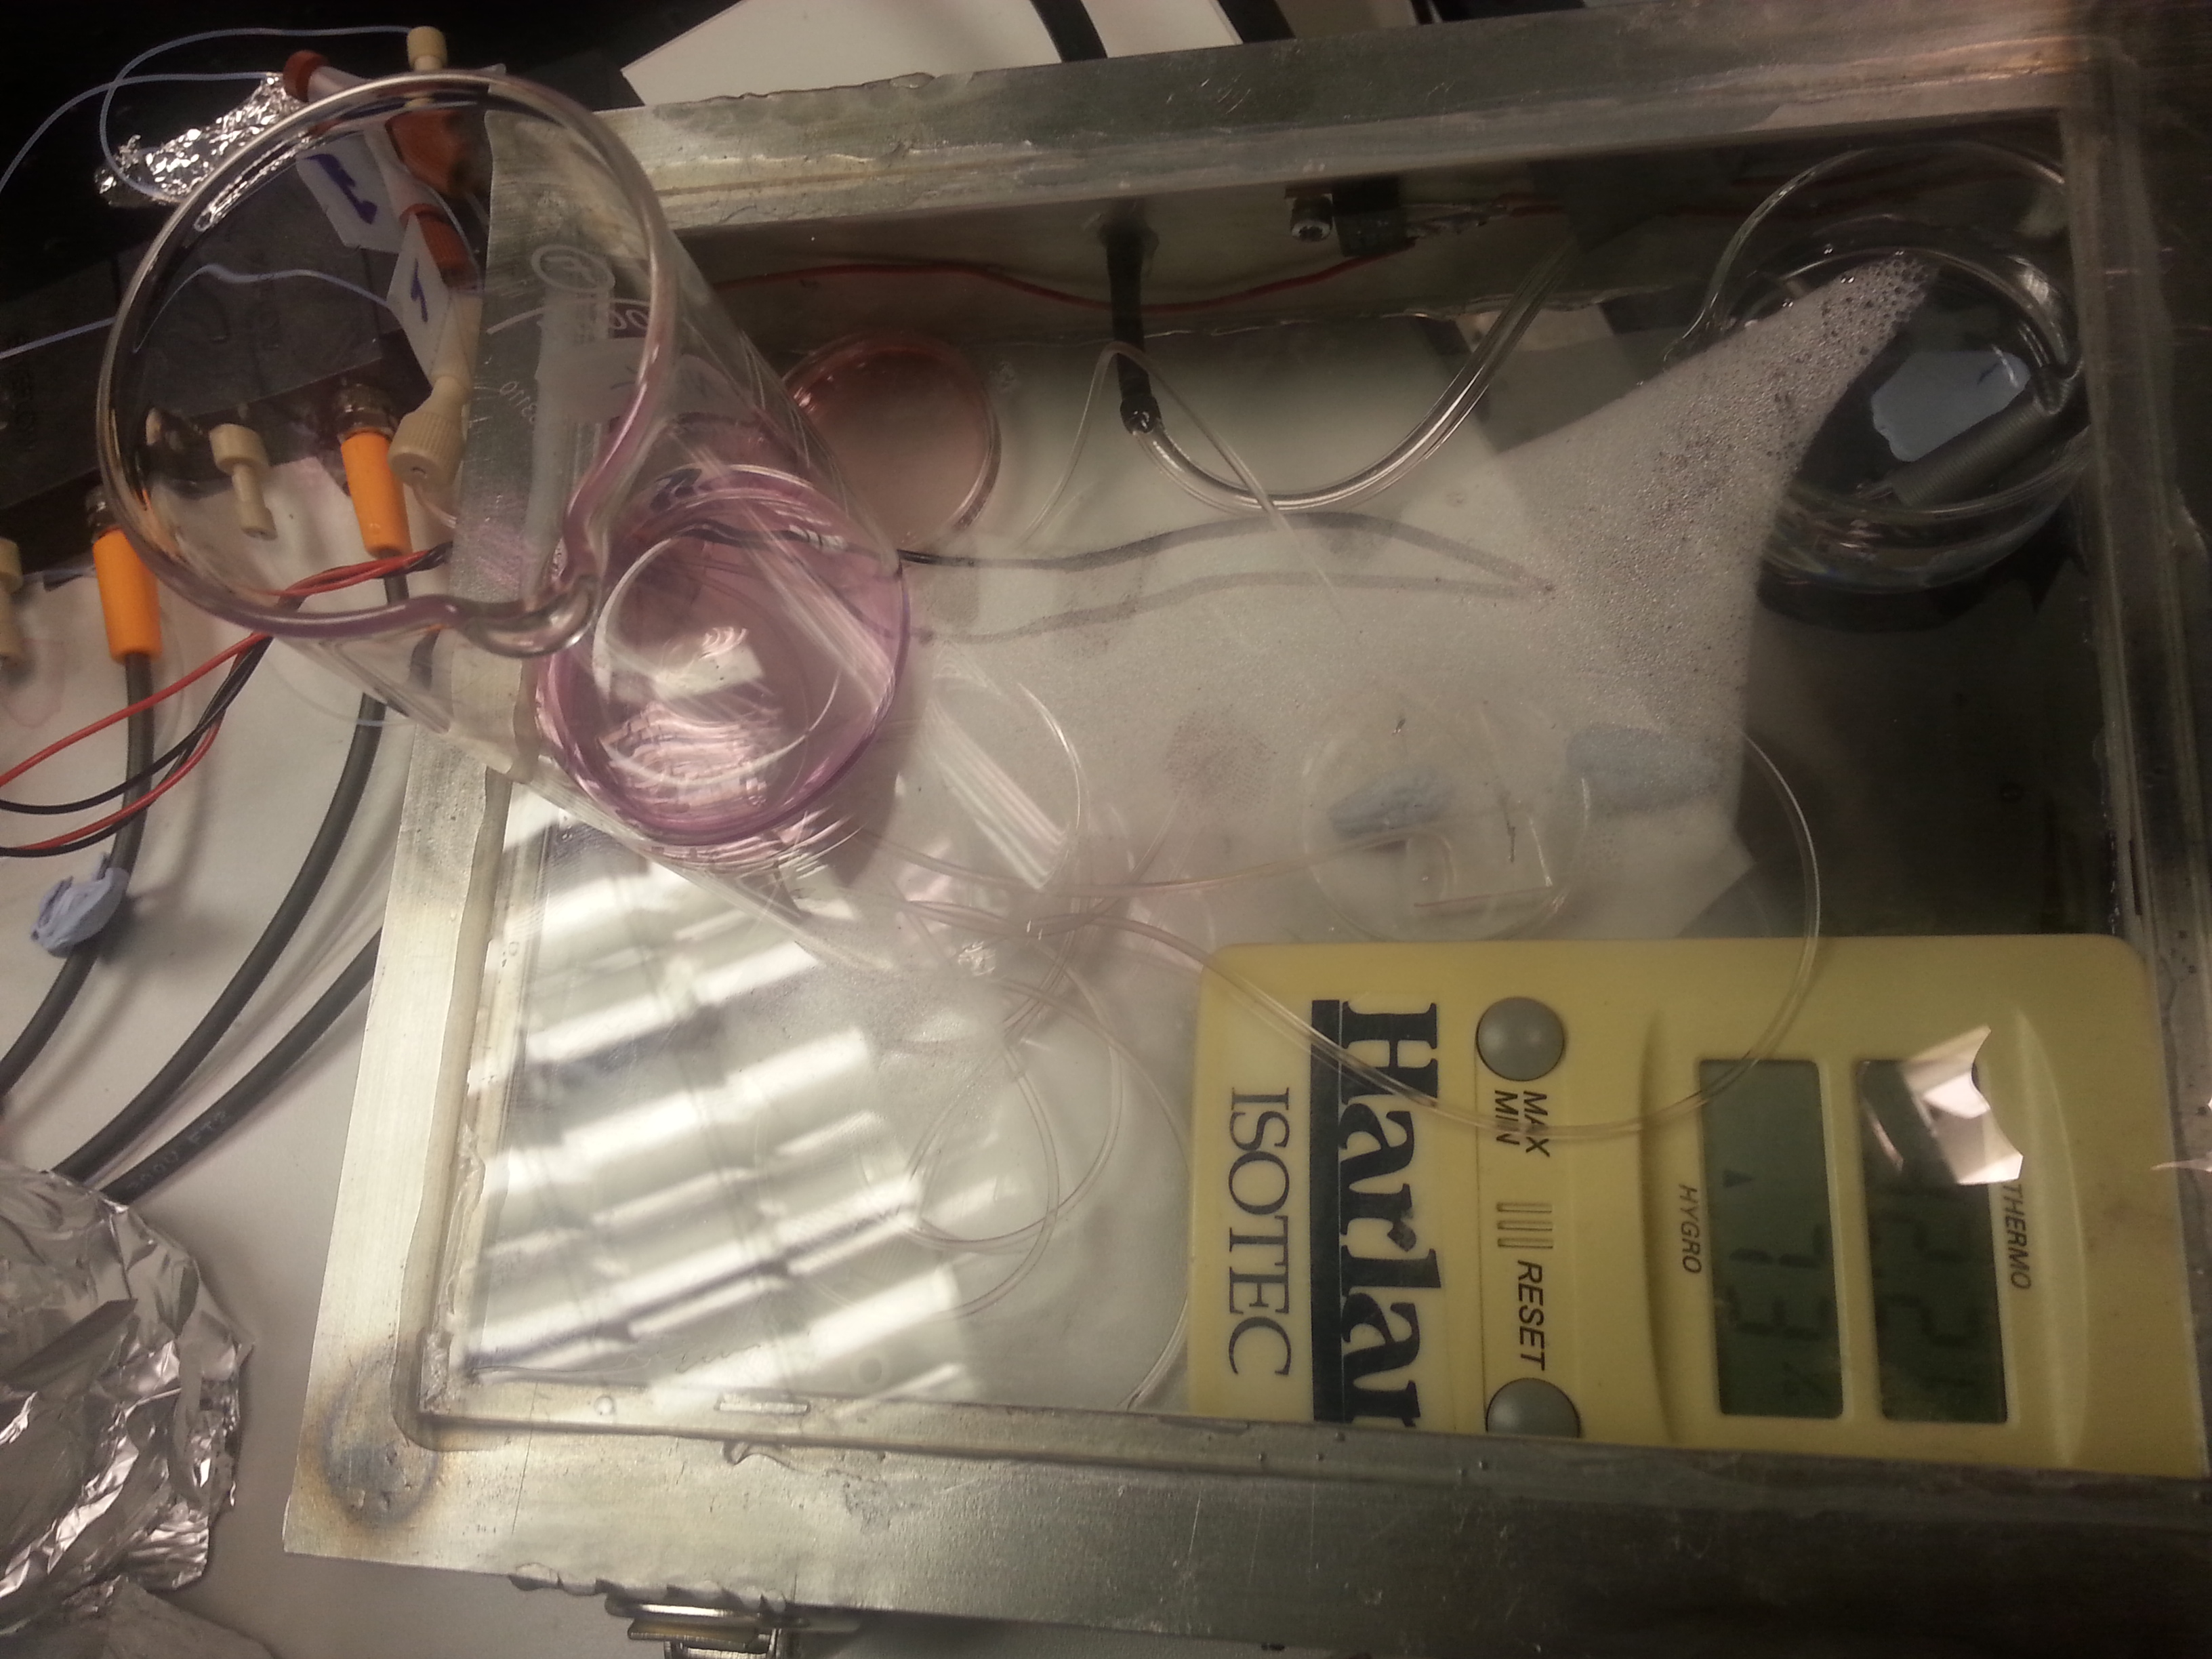
\includegraphics[width=15cm]{chapter2/figures/Chamber/ChamberInOperation.jpg}
            \caption[Image of environmental chamber]{\textbf{Environmental chamber is able to maintain physiological temperature and CO\textsc{2} levels.} Image shows environmental chamber during process of heating up. The level of CO\textsc{2} saturation is indicated by the color of the media which contains Phenol Red. A beaker with media outside the chamber is shown as a non-CO\textsc{2}-saturated color reference. The media inside the chamber is observably more basic.}
            \label{fig:app:chamber}

        \end{figure}
        
        \begin{figure}[h]
           \centering
            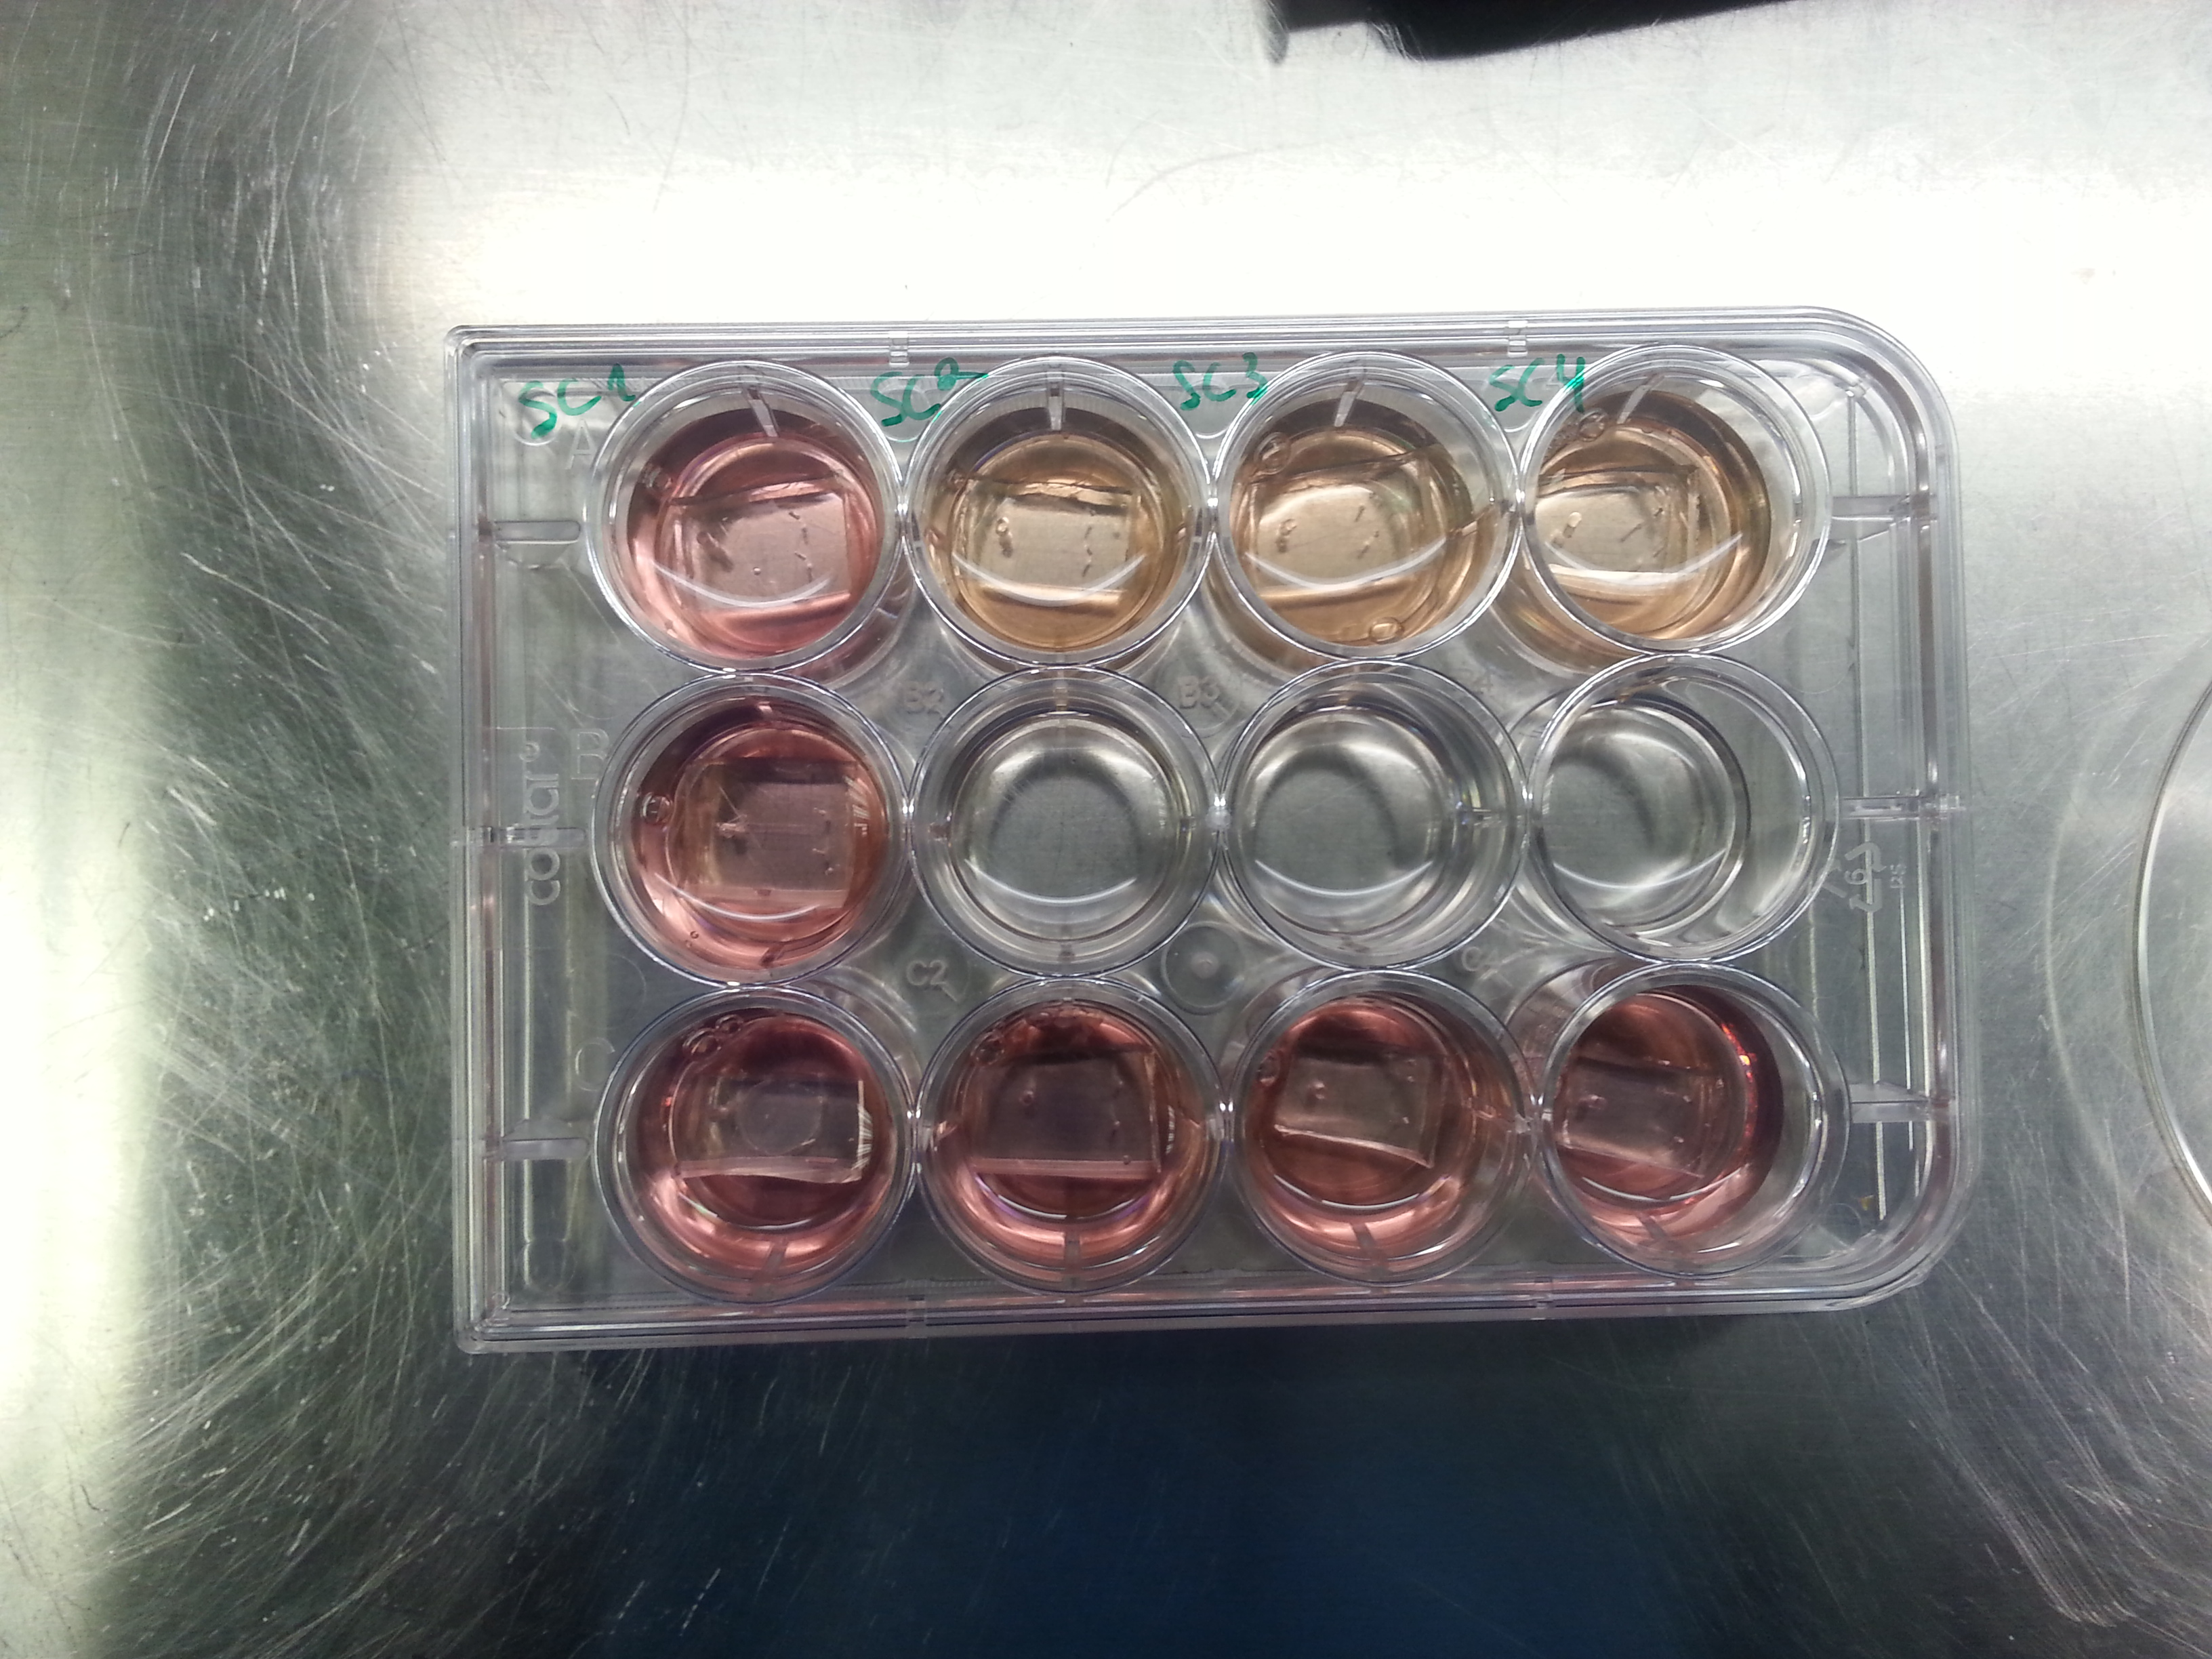
\includegraphics[width=12cm]{chapter4/figures/immersionMethod/12WellImmersion.jpg}
            \caption[The immersion maintenance configuration]{\textbf{The immersion configuration.} In this configuration, the devices were immersed in 12-wells with \(2.5-3 ml\) media each to prevent excessive osmotic drifts. This configuration required immersion 24 hours prior to seeding to release air trapped in the PDMS.}
            \label{fig:devices:immersion}
        \end{figure}

        \begin{figure}[!h]
            \centering
            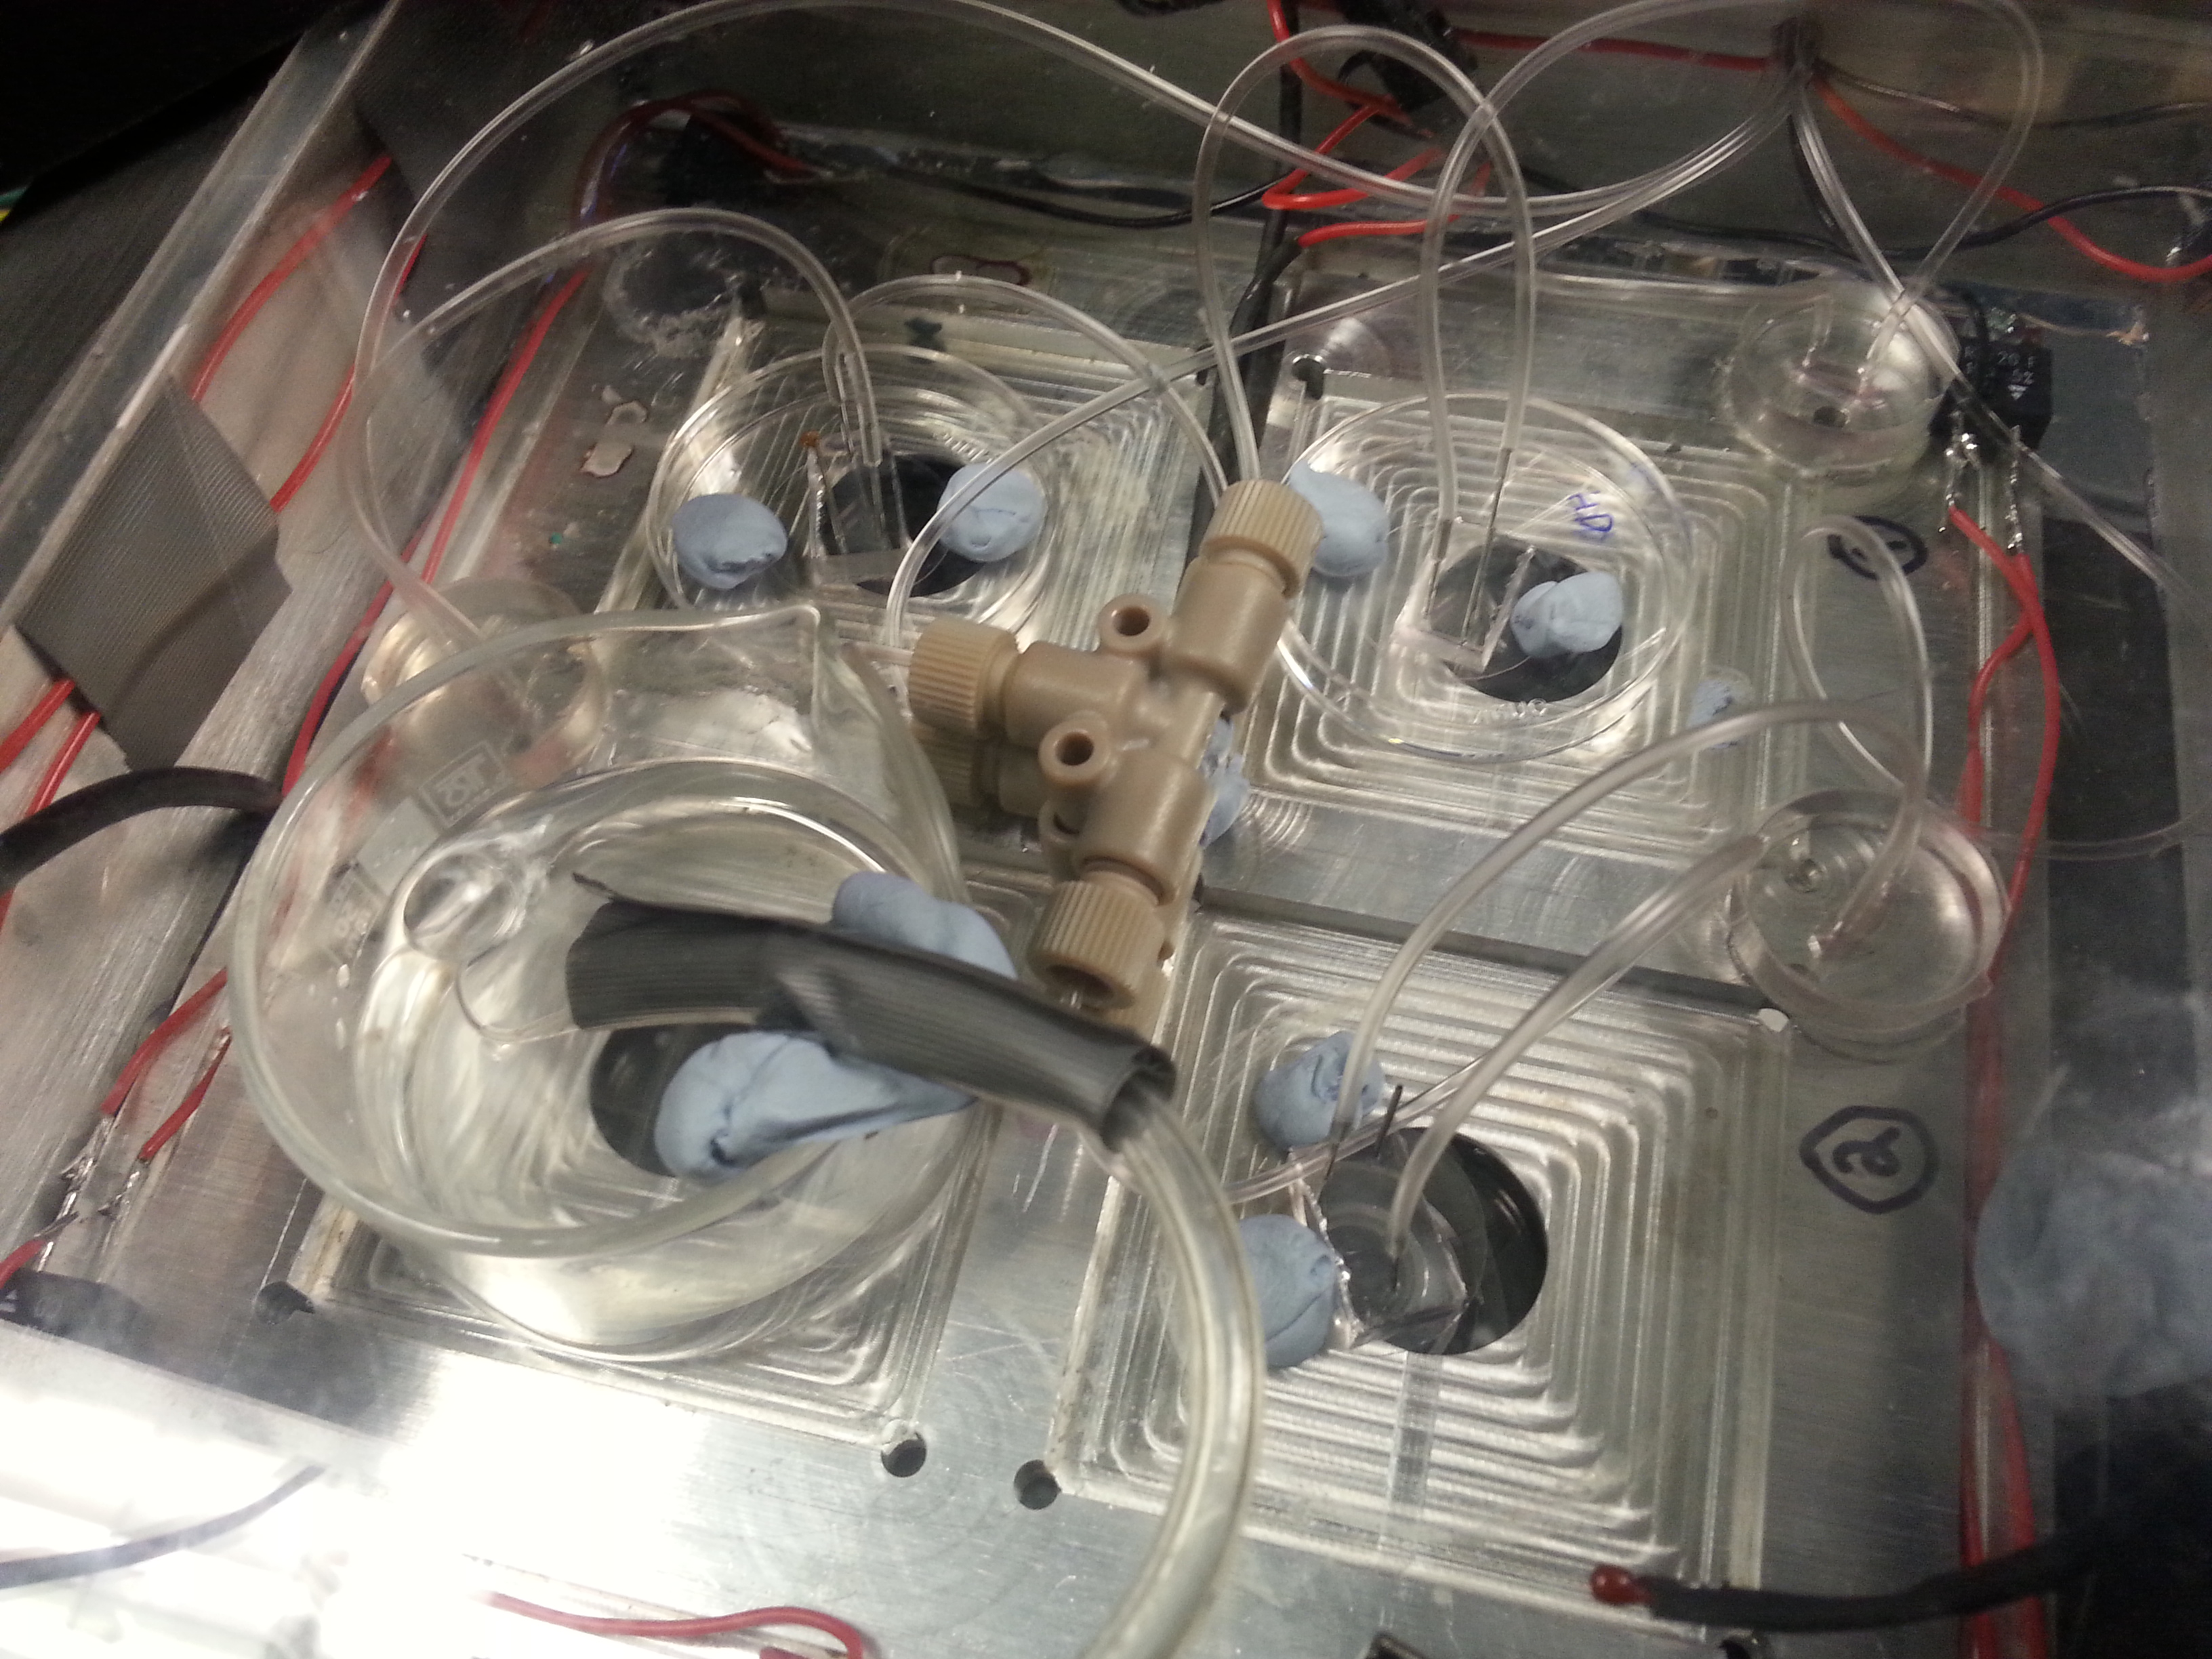
\includegraphics[width=15cm]{chapter2/figures/flow/3Devices.jpg}
            \caption[Image of 3 coverslip devices under flow simultaneously]{\textbf{Up to 3 devices may be simultaneously connected to independent flow channels.}}
            \label{fig:app:3Devices}

        \end{figure}

        \begin{SCfigure}
            \centering
            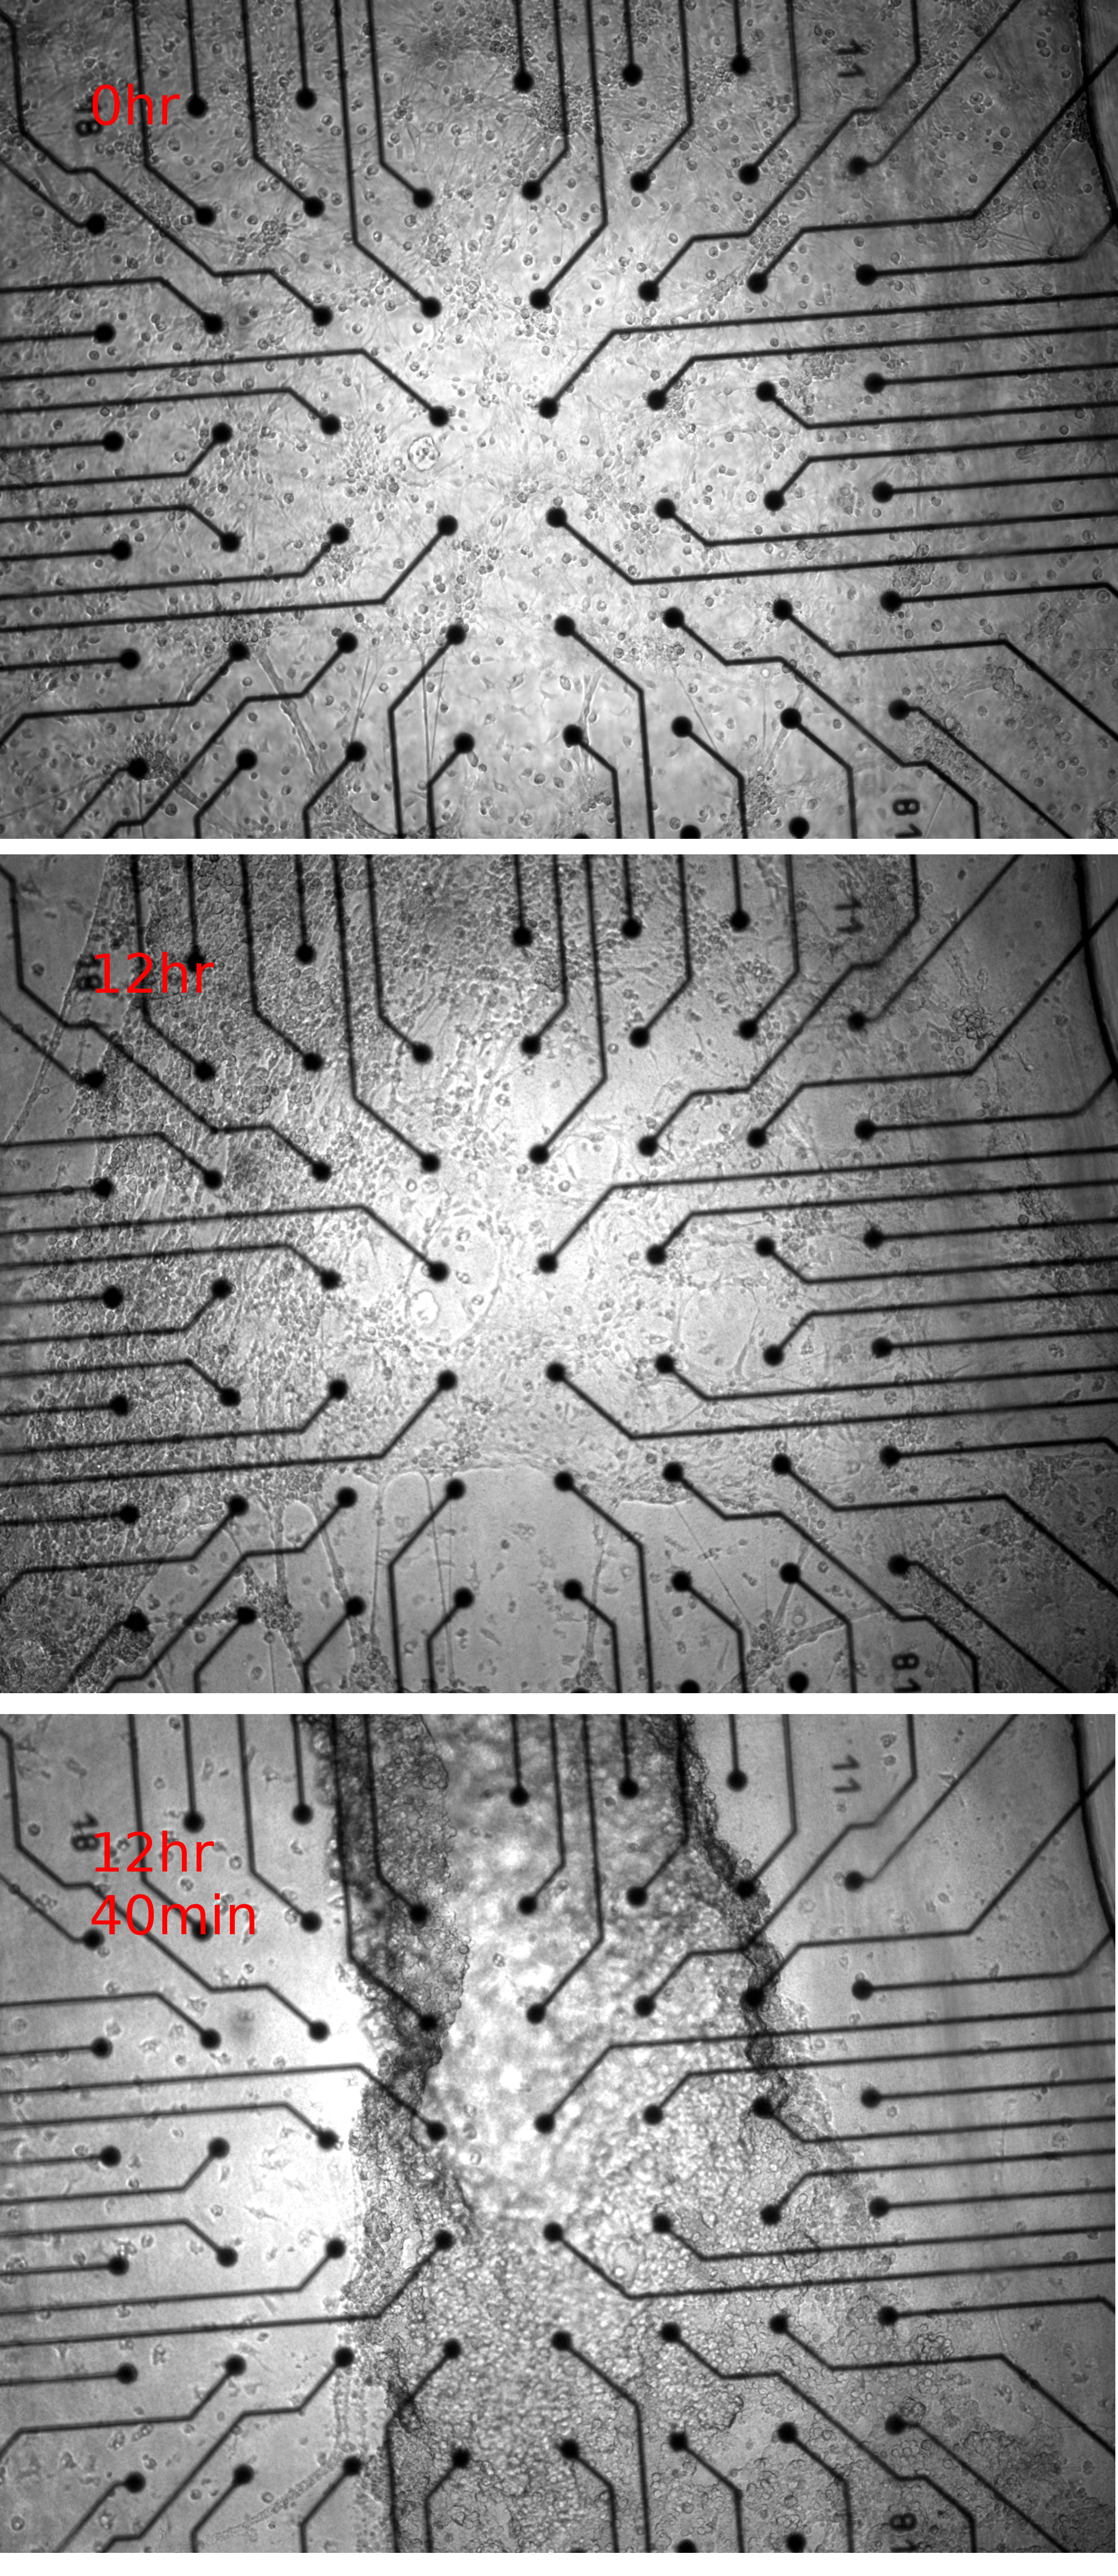
\includegraphics[width=10.5cm]{appendix/tissueDetachment/tissueDet.jpg}
            \caption[Time lapse of culture under flow exhibiting complete tissue detachment]{\textbf{Older cultures subjected to flow detached as a single sheet of tissue.} Time lapse images of a 10 days \textit{in vitro} culture, grown on an MEA surface and placed under flow with a flow rate setting of \(0\frac{nl}{s}\).}
            \label{fig:app:culturePeel}

        \end{SCfigure}

        \begin{figure}[h]
            \centering
            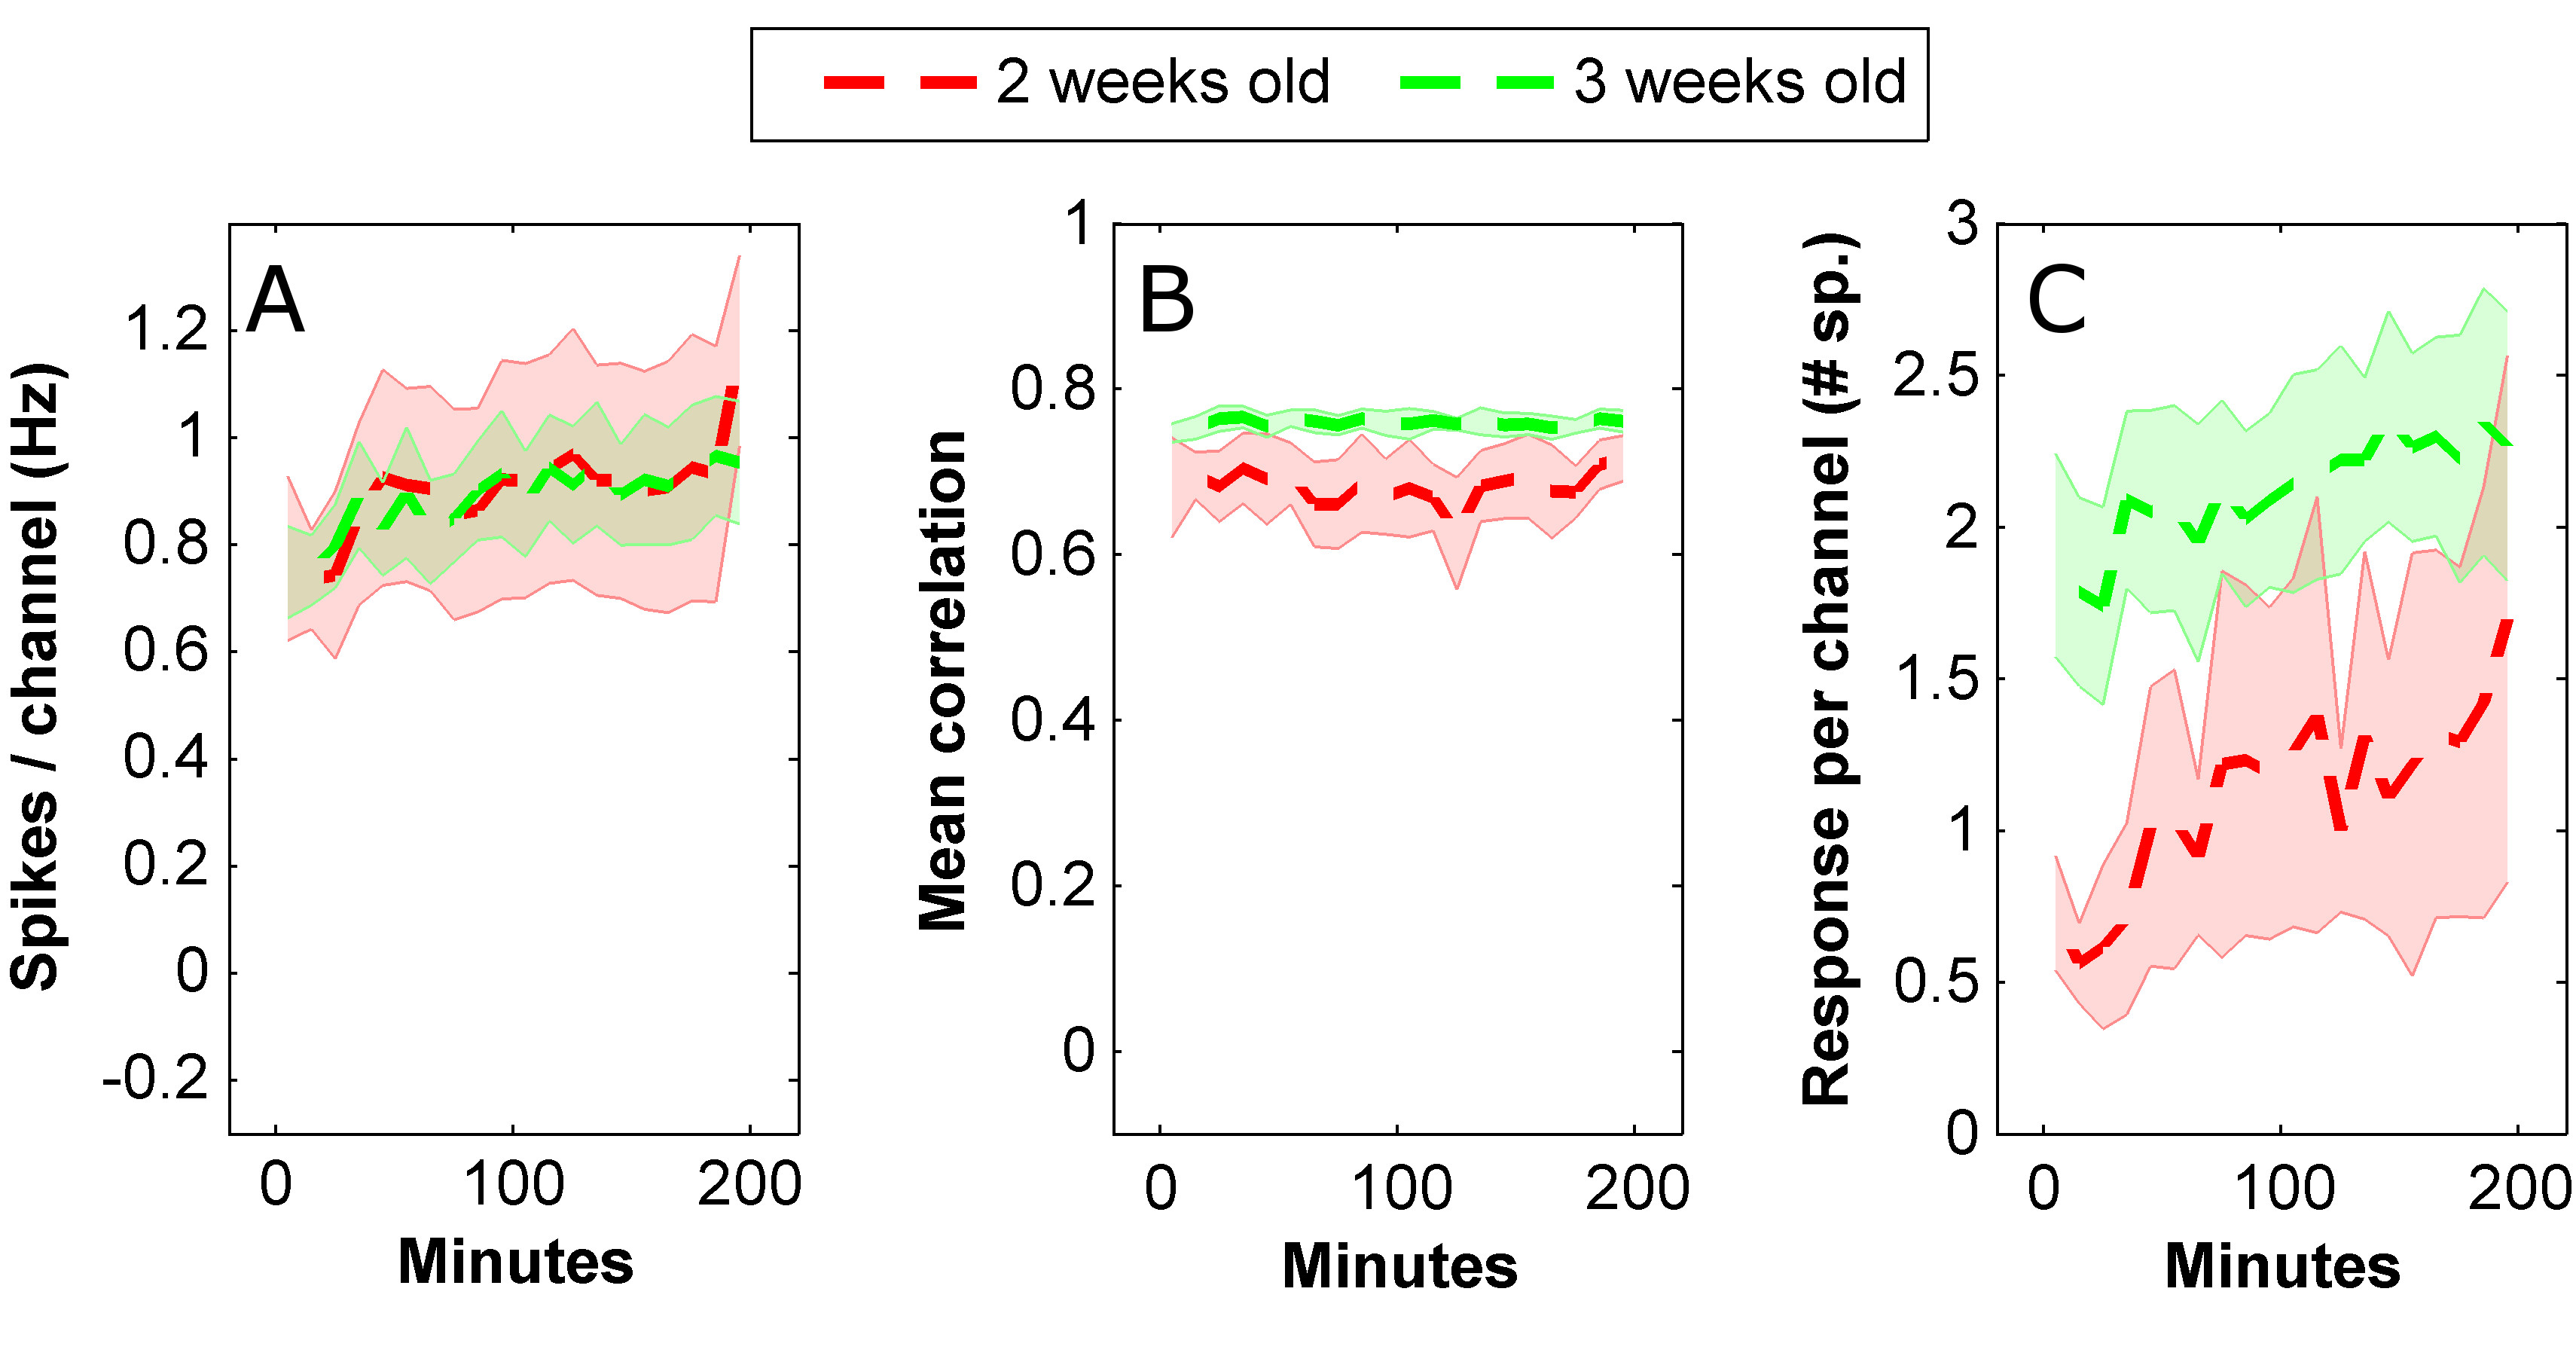
\includegraphics[width=14.5cm]{appendix/youngOldCompare.jpg}
            \caption[Comparison of activity measures for 2 and 3 week old cultures]{\textbf{Activity in 3 weeks old cultures is less variable and their stimulation response is twice as intense compared to 2 weeks old cultures.} Figure shows the control curves (experiments without flow) from figure \ref{fig:crossFlow:youngOldStats}. In this case the firing rate (A) and stimulation response (C) data are not normalized (note y-axis units) to allow direct comparison between the two age groups.}

            \label{fig:app:youngOldCompare}

        \end{figure}

        \begin{figure}[!htb]
            \centering
            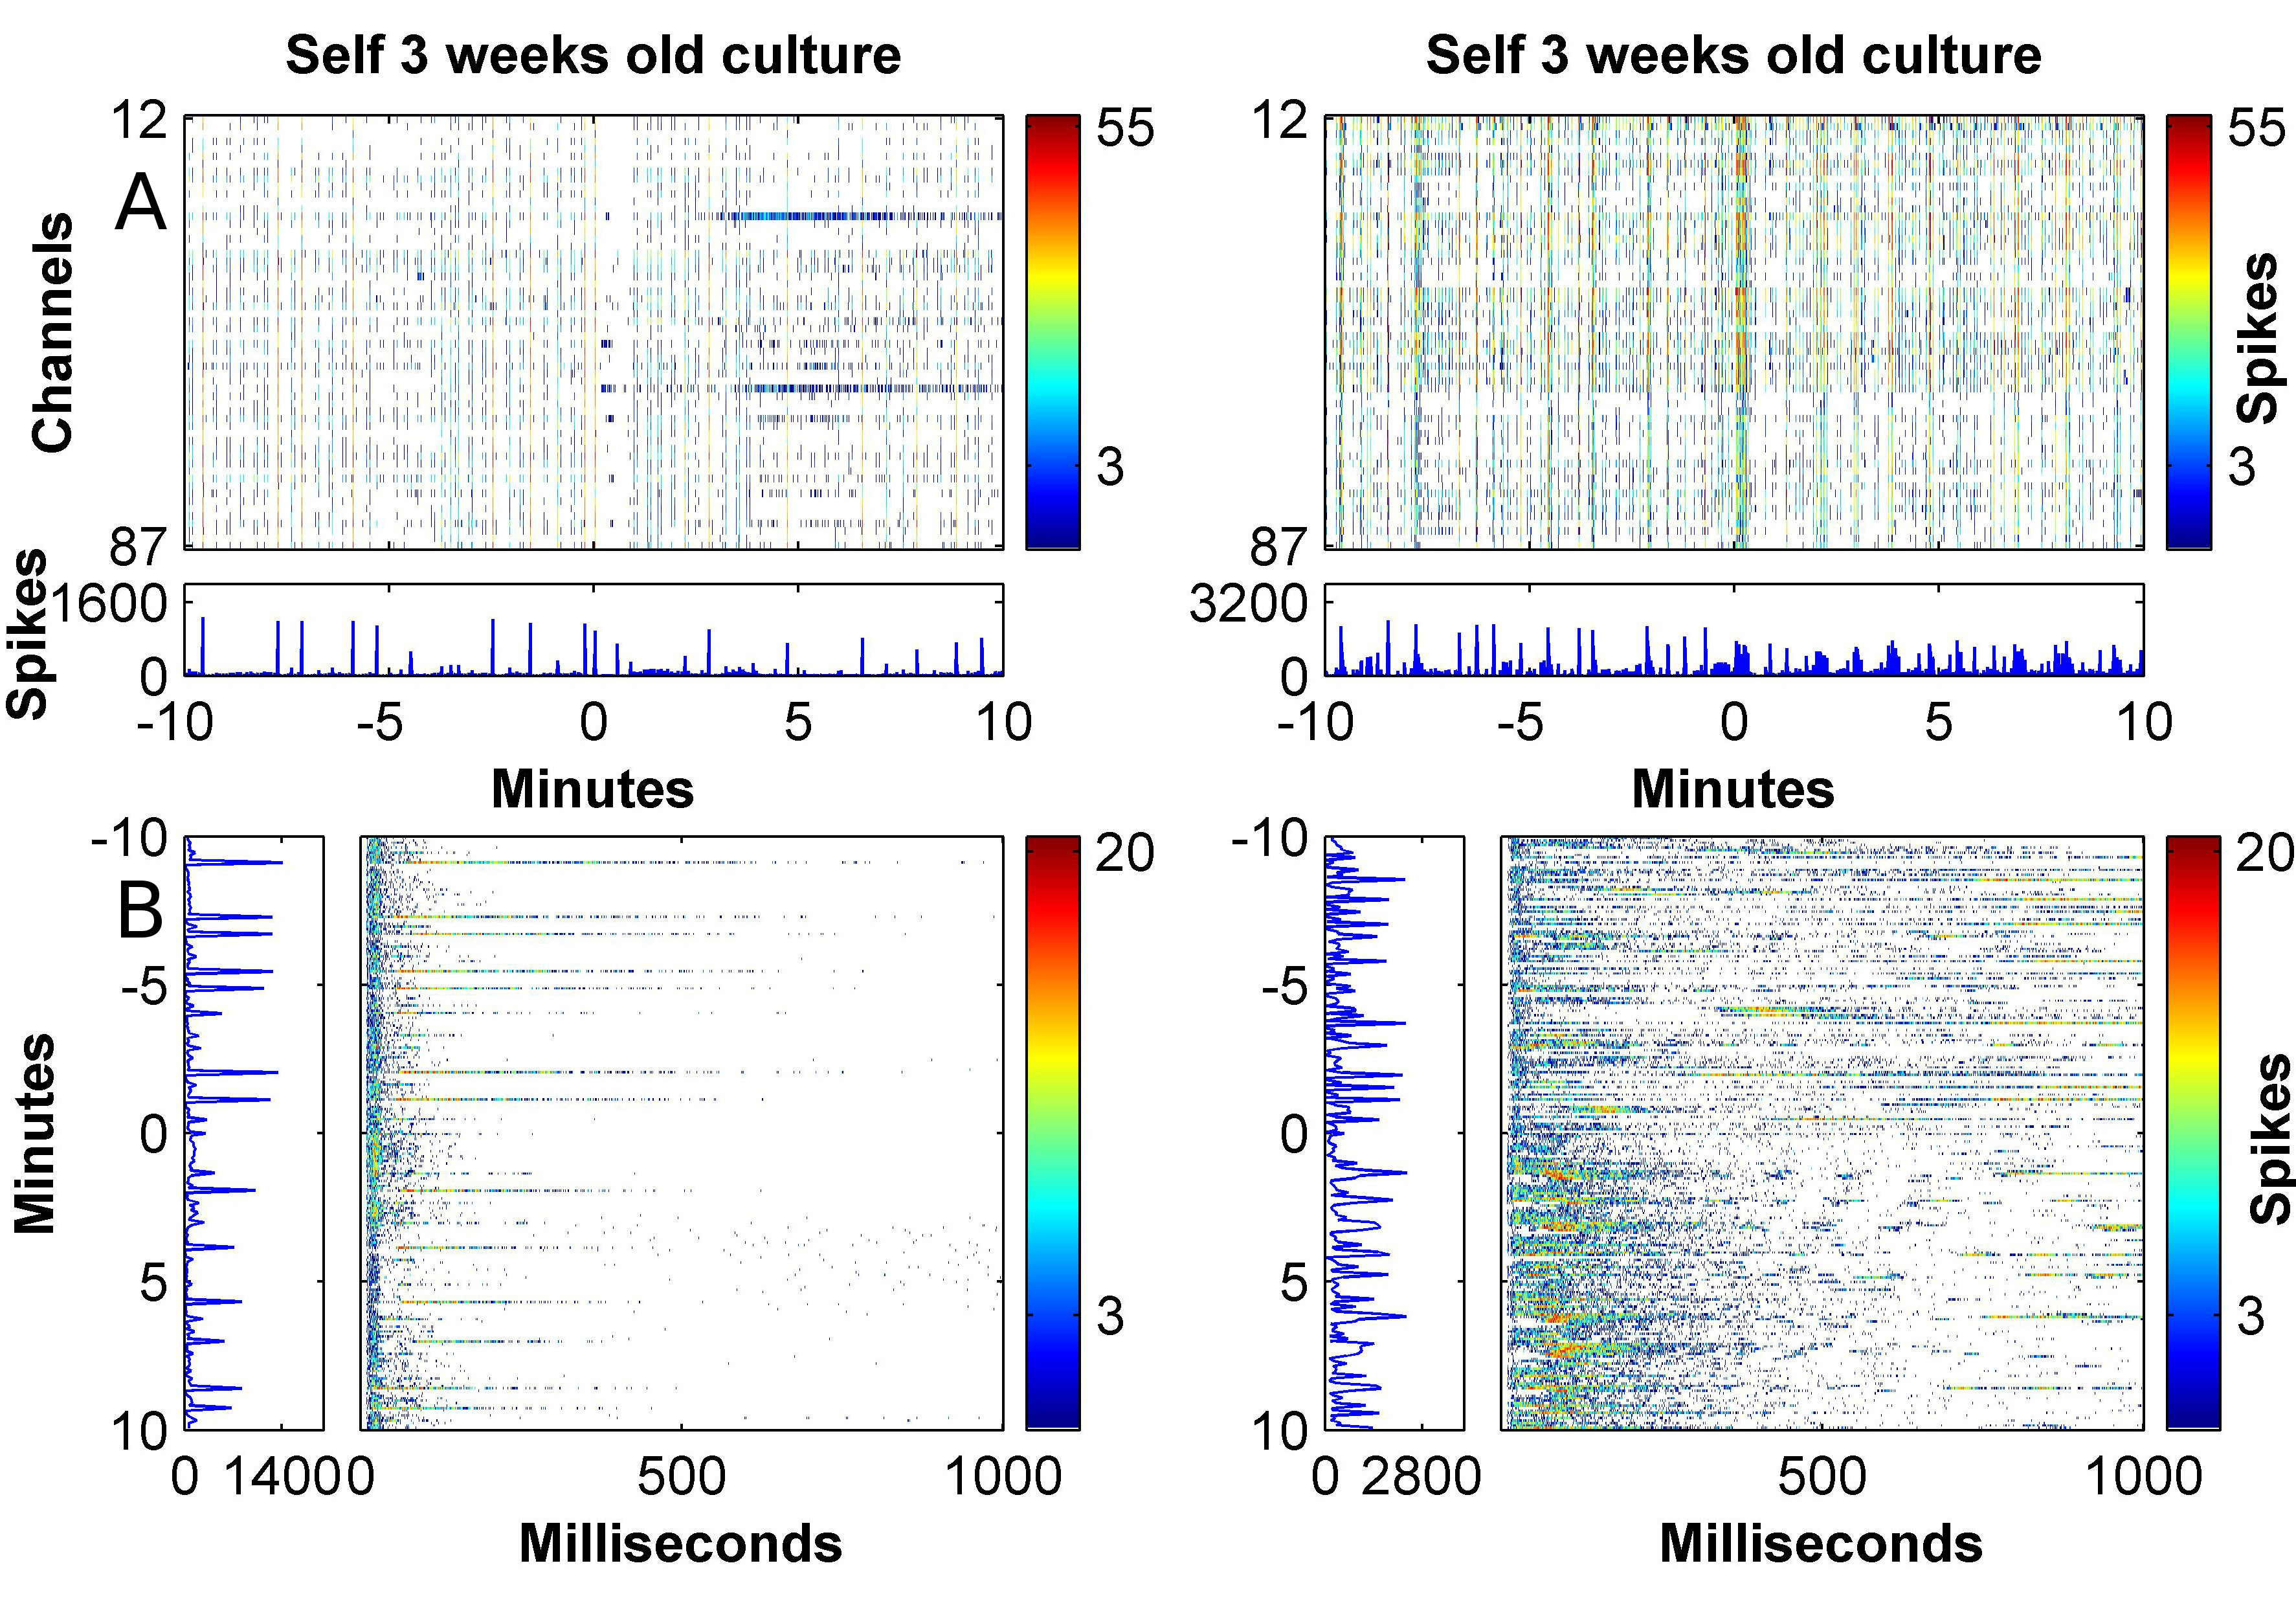
\includegraphics[width=15cm]{chapter5/figures/moreOldExamples/moreOldRasterExamples.jpg}
            \caption[Further examples for 3 weeks old cultures under flow with self media]{\textbf{3 week old cultures maintain network function under flow with self media.} Data presented as in figure \ref{fig:crossFlow:slowFastExample} In this case the activity and stimulation responses are maintained under fast flow although some modulations are observed.}
            \label{fig:crossFlow:moreOldExamplesRaster}
        \end{figure}

